\documentclass{article}
\usepackage[a4paper,margin=3cm,footskip=.5cm]{geometry}
\usepackage{amsmath,amssymb,amsthm,amsfonts,mdframed,kotex}
\newcounter{num}
\newcommand{\bp}
{\stepcounter{num}
\begin{mdframed}
[frametitle={\thenum},skipabove=10pt,skipbelow=10pt]}
\newcommand{\ep}
{\vspace{0.1\textheight}
\par
\end{mdframed}}
\newcommand{\parall}{\mathbin{\!/\mkern-5mu/\!}}
\mdfsetup{nobreak=true}

\title{혜령 : 04 2013년 6월 모의고사 12번, 27번(3학년 1학기)(1)}
\date{\today}
\author{}

\begin{document}
12.

\begin{figure}[h]
\centering
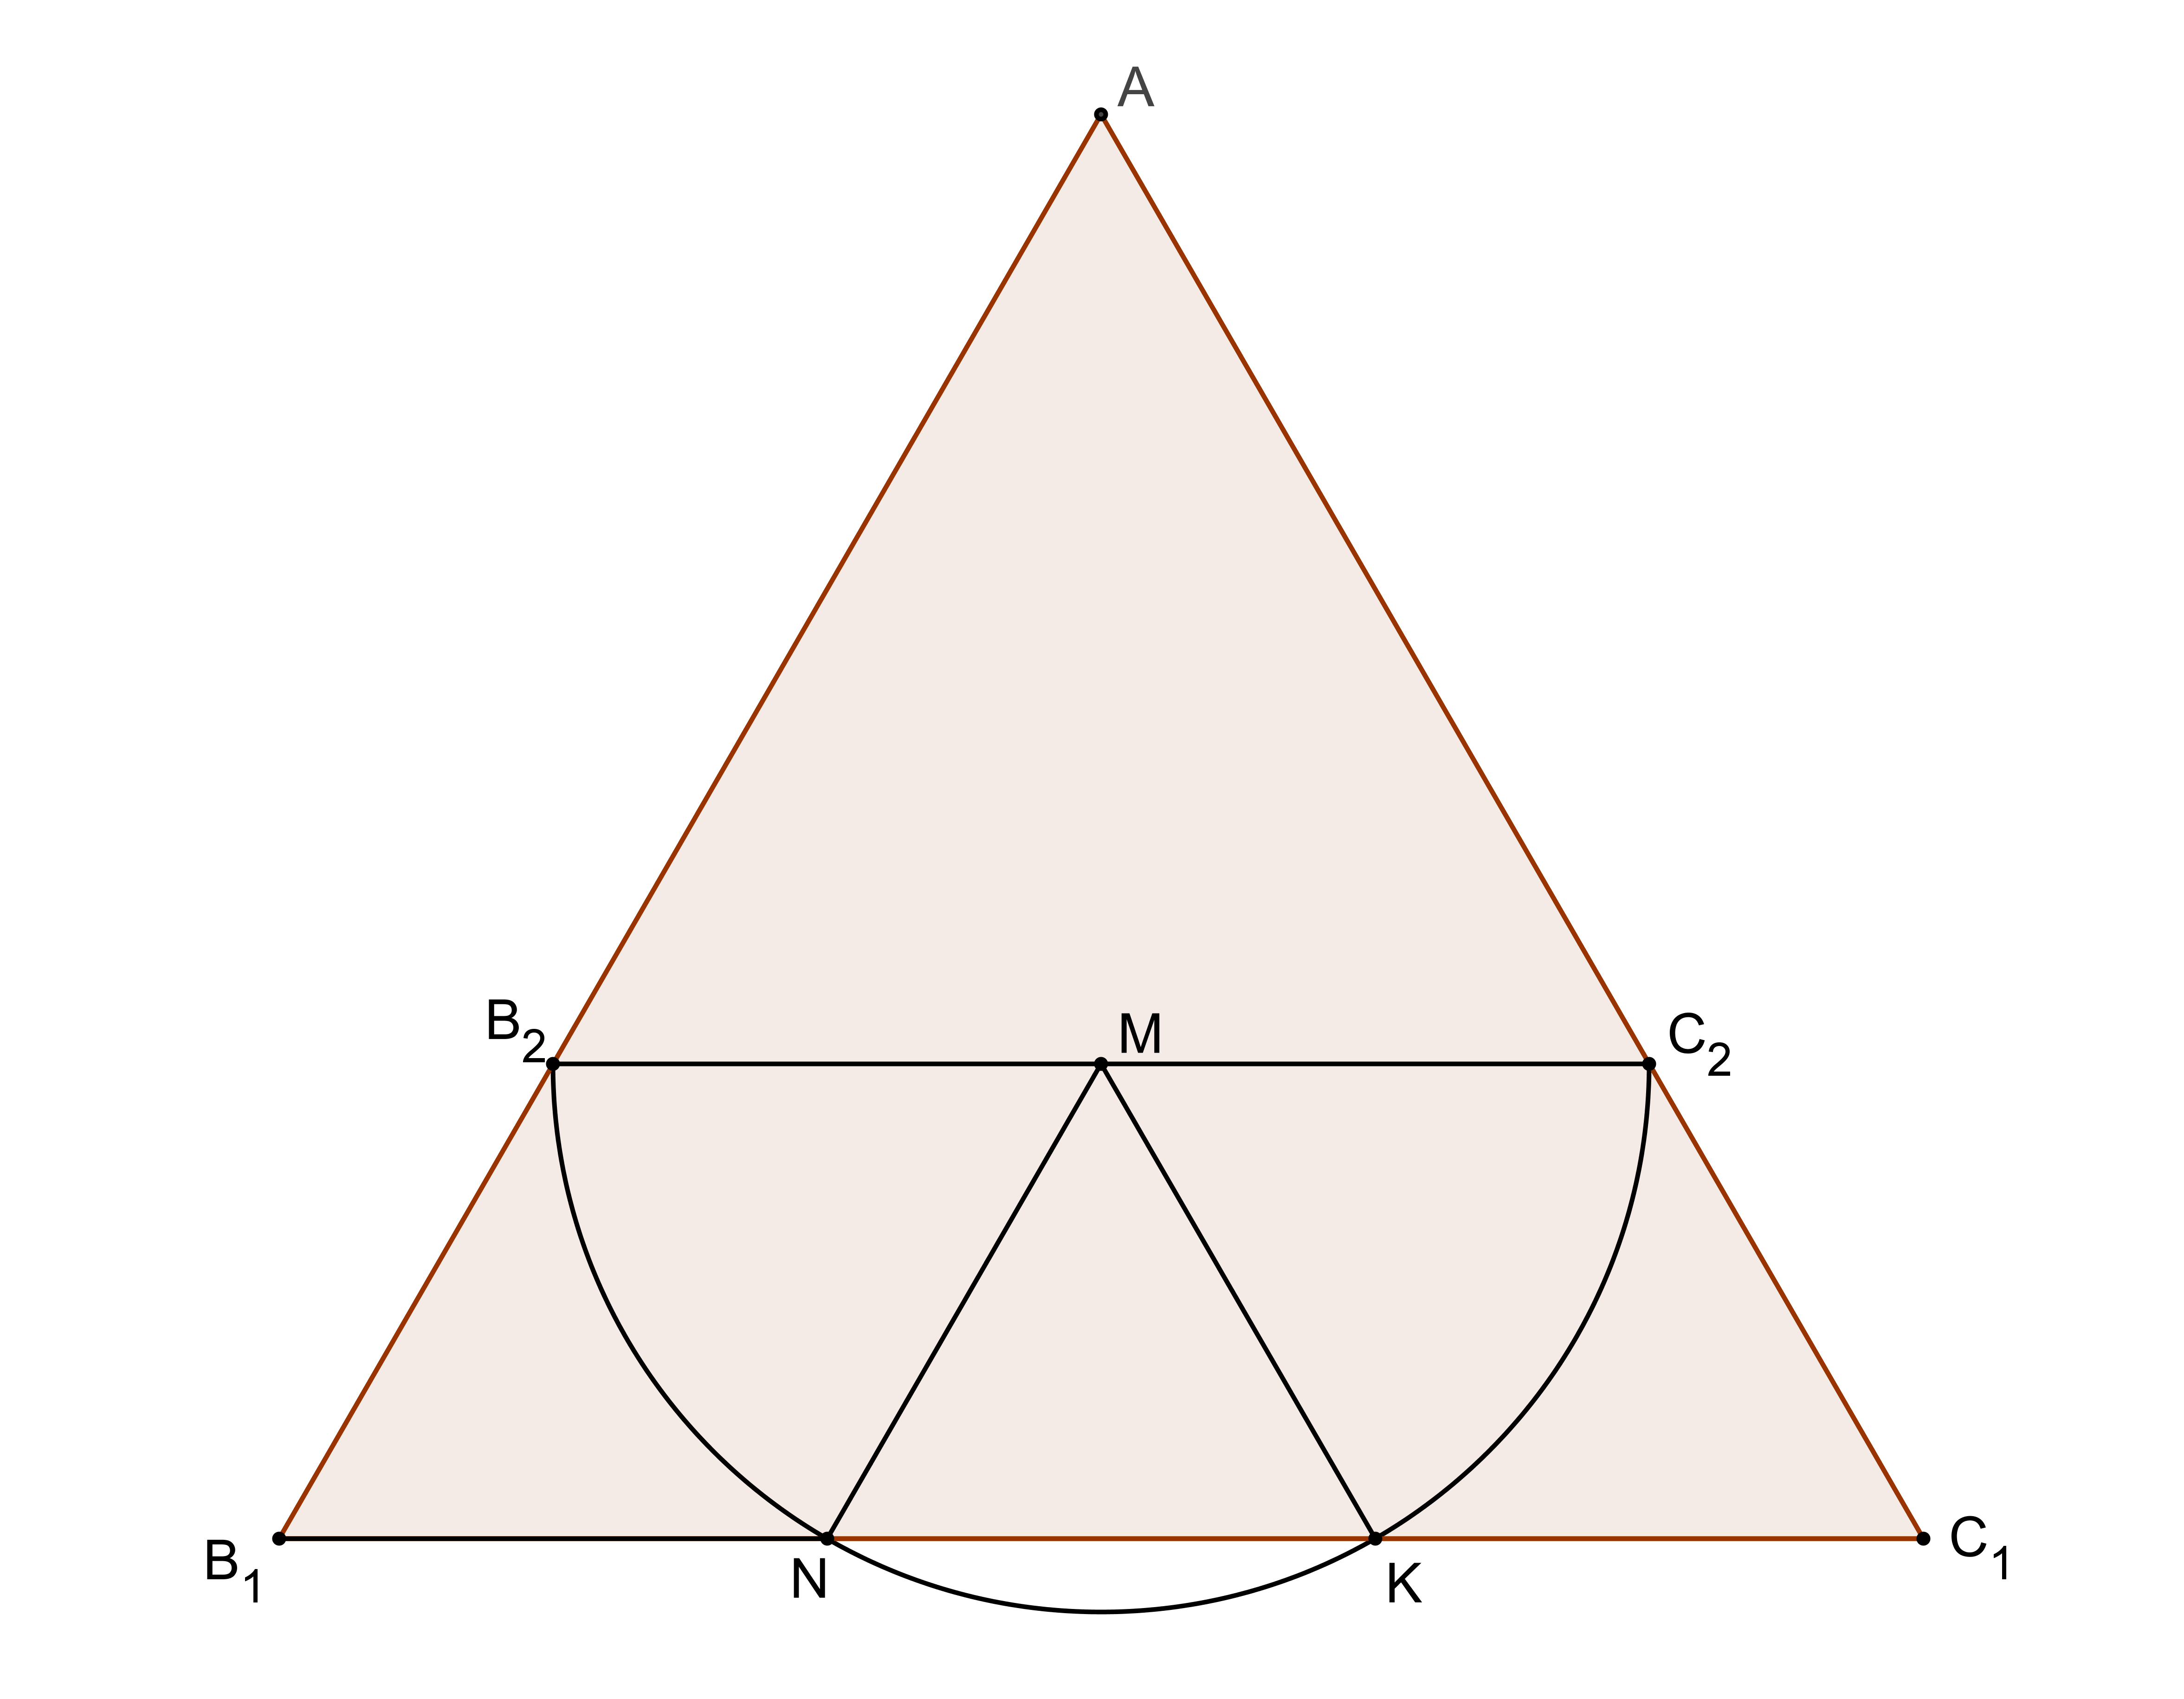
\includegraphics[width=0.5\textwidth]{12}
\end{figure}

\(B_1B_2=1\), \(MN=1\), \(\therefore B_1B_2=MN\).
또 \(B_2M\parall B_1N\).
한 쌍의 대변의 길이가 같고 다른 한 쌍의 대변이 서로 평행하므로 \(\square MNB_1B_2\)는 평행사변형이거나 등변사다리꼴이다.
그런데 등변사다리꼴은 아니므로 평행사변형이다.
따라서 \(B_1N=1\)이다.
마찬가지로 \(C_1K=1\)이다.
그러므로 \(NK=1\)이고 따라서 삼각형 \(MNK\)는 정삼각형이다.

\(S_1\)을 계산해보면
\begin{gather*}
부채꼴 NMK=\frac12\times1^2\times\frac\pi3=\frac\pi6.\\
\triangle NMK=\frac{\sqrt3}4\times1^2=\frac{\sqrt3}4.\\
S_1=\frac\pi6-\frac{\sqrt3}4.
\end{gather*}

한편 \(\triangle AB_1C_1\sim\triangle AB_2C_2\)이고 이 때의 닮음비는 3:2이다.
따라서 \((S_1\text{의 모양})\sim(S_2\text{의 모양})\)이고 이 떄의 닮음비도 3:2이다.
그러므로 \(\frac{S_2}{S_1}=\frac49\).
\(\{S_n\}\)은 첫항이 \(\frac\pi6-\frac{\sqrt3}4\)이고 공비가 \(\frac49\)인 등비수열이다.

\[\sum_{n=1}^\infty S_n=\frac{\frac\pi6-\frac{\sqrt3}4}{1-\frac49}=\frac{6\pi-9\sqrt3}{20}\]

\begin{mdframed}[leftmargin=0.91\textwidth,innerleftmargin=5pt]
답:2번
\end{mdframed}
\newpage

27.

\begin{figure}[h]
\centering
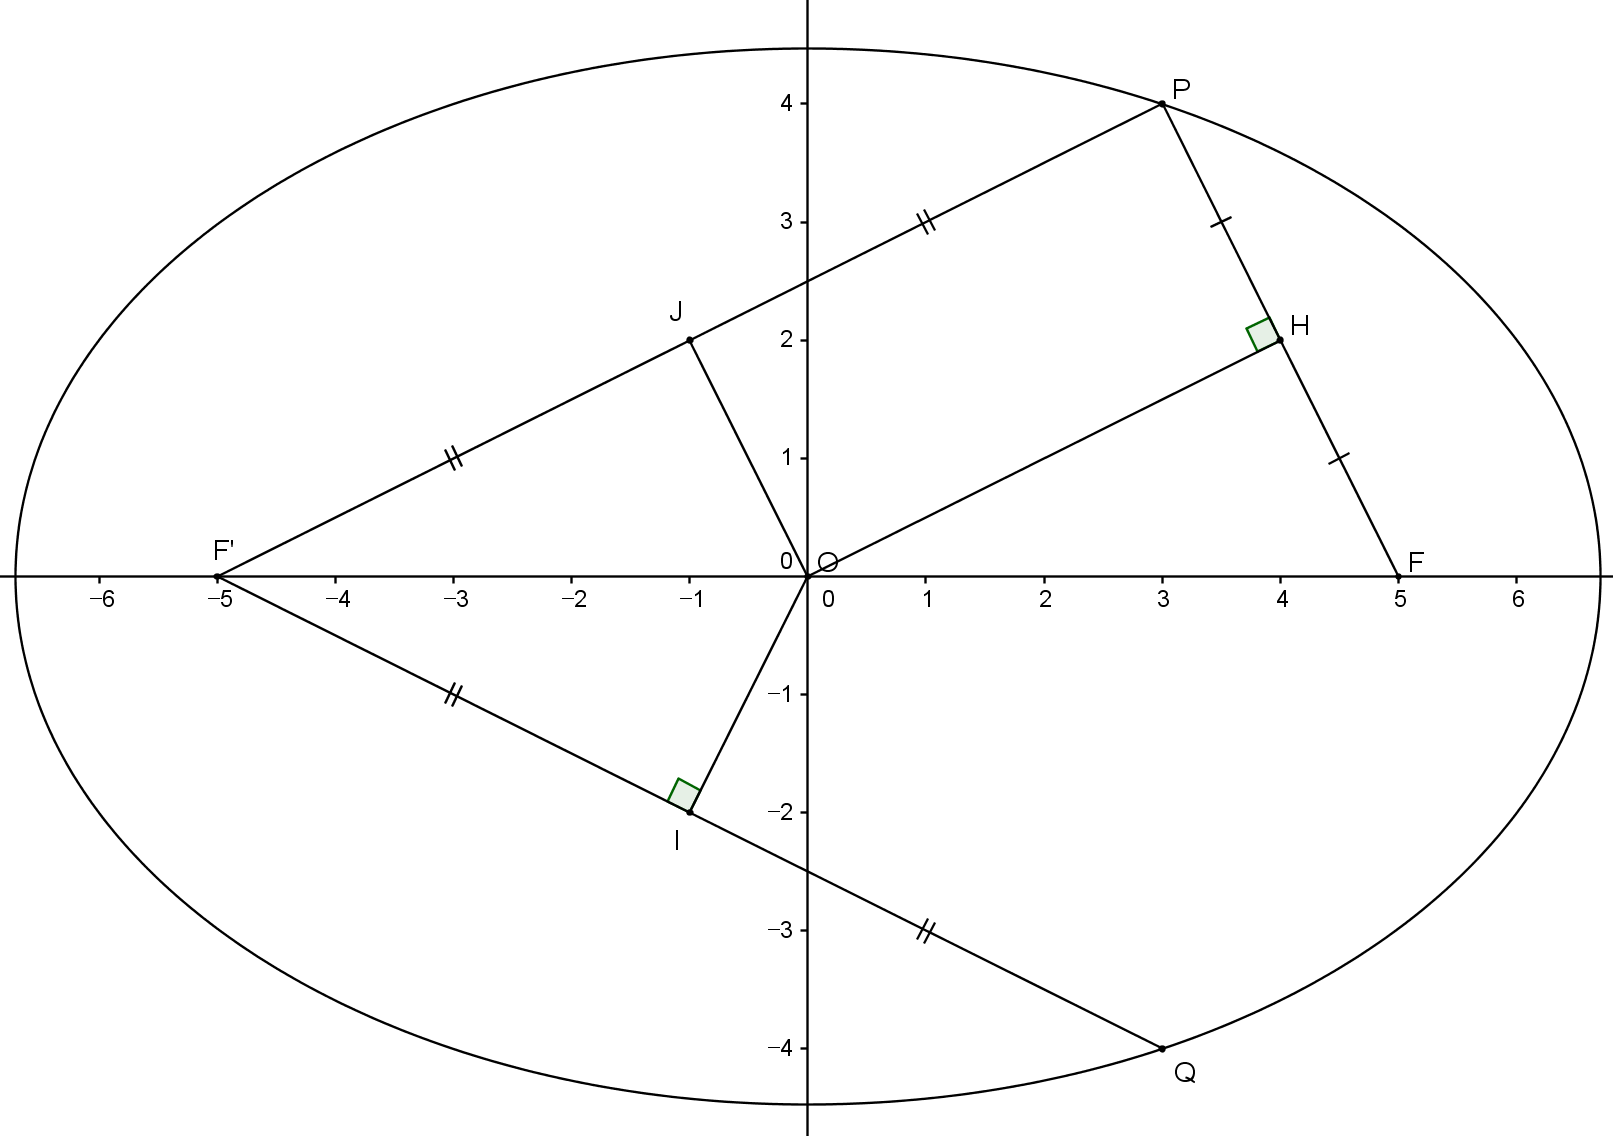
\includegraphics[width=0.8\textwidth]{27}
\end{figure}

\(\triangle OIF'\equiv\triangle OIQ\)에서 \(OQ=5\).
\(\triangle OHF\equiv\triangle OHP\)에서 \(OP=5\).
따라서 \(OQ=OP\)이므로 \(P\)와 \(Q\)는 서로 \(x\)축 대칭이다.
\(I\)를 \(x\)축 대칭이동시킨 점을 \(J\)라고 하고 \(PF'=m\), \(PF=n\)이라고 하면,
\[mn=2\overline{OH}\times2\overline{OJ}=40.\]
한편 \(P\)는 지름이 \(F'F\)인 원 위에 있으므로 \(\angle F'PF=90^\circ\).
따라서
\[m^2+n^2=\overline{F'F}^2=100.\]
그러므로
\[(m+n)^2=100+2\times 40=180.\]
\(l=\text{장축의 길이}=m+n=\sqrt{180}\).
\(\therefore l^2=180.\)


\begin{mdframed}[leftmargin=0.91\textwidth,innerleftmargin=5pt]
답:180
\end{mdframed}

\end{document}